\documentclass{article}%
\usepackage[T1]{fontenc}%
\usepackage[utf8]{inputenc}%
\usepackage{lmodern}%
\usepackage{textcomp}%
\usepackage{lastpage}%
\usepackage[head=40pt,margin=0.5in,bottom=0.6in]{geometry}%
\usepackage{graphicx}%
%
\title{\textbf{Profesores y personal de la ULA exigieron seguridad en la institución}}%
\author{El Nacional Web}%
\date{19/11/2018}%
%
\begin{document}%
\normalsize%
\maketitle%
\textbf{URL: }%
http://www.el{-}nacional.com/noticias/protestas/profesores{-}personal{-}ula{-}exigieron{-}seguridad{-}institucion\_260297\newline%
%
\textbf{Periodico: }%
EN, %
ID: %
260297, %
Seccion: %
Protestas\newline%
%
\textbf{Palabras Claves: }%
Mérida, Protestas, Sociedad\newline%
%
\textbf{Derecho: }%
2.2, %
Otros Derechos: %
, %
Sub Derechos: %
2.2.1\newline%
%
\textbf{EP: }%
SI\newline%
\newline%
%
\textbf{\textit{Un grupo de personas rechazó el robo y la agresión de las que fue víctima un vigilante de la universidad}}%
\newline%
\newline%
%
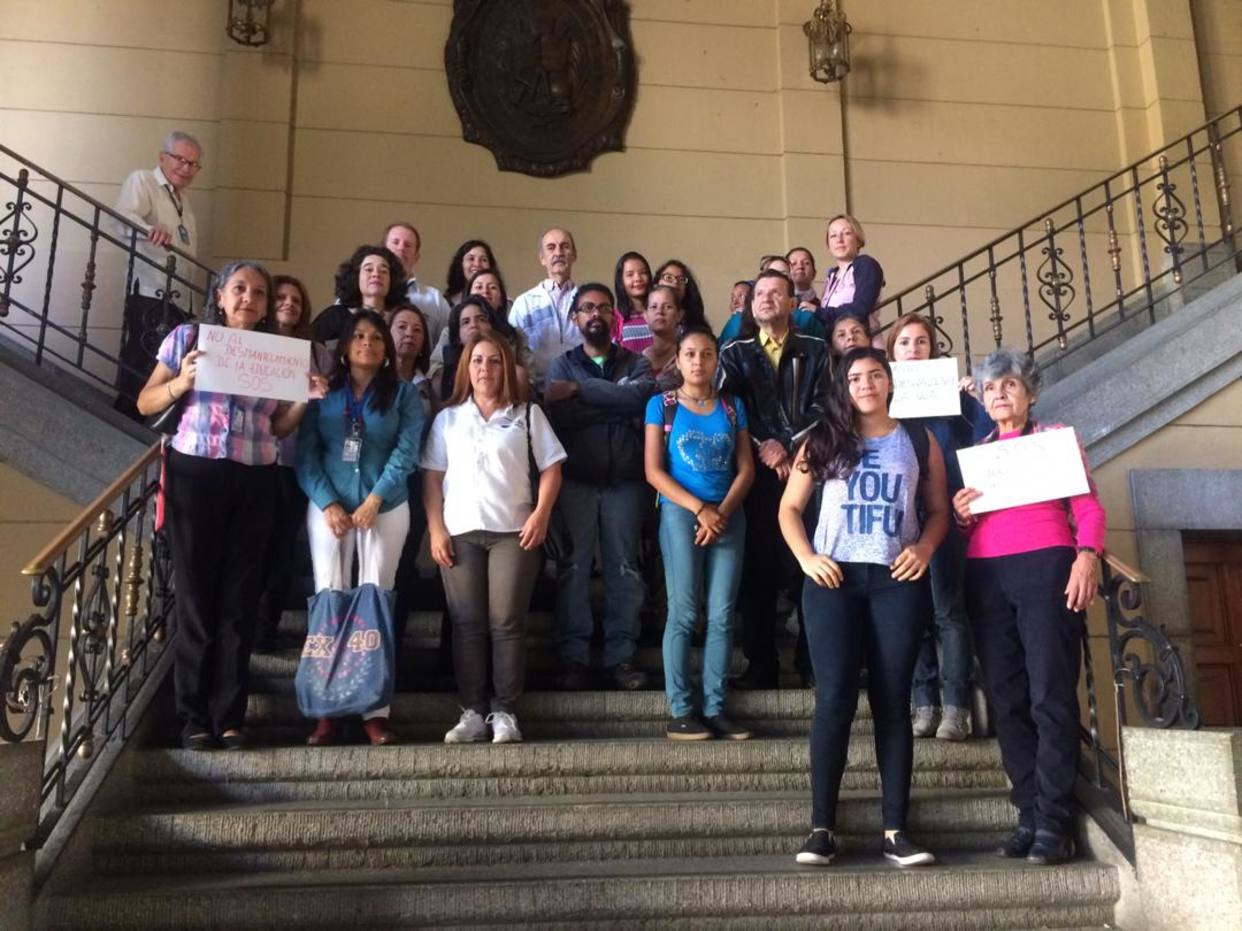
\includegraphics[width=300px]{48.jpg}%
\newline%
%
Un grupo de profesores y del personal de la Facultad de Humanidades y Educación de la Universidad de los Andes (ULA), ubicada en el estado Mérida, exigió protección ante los hechos de violencia registrados en su dependencia.%
\newline%
%
El corresponsal de~El Nacional~en la entidad, Leonardo León, dijo que las personas aseguran que requieren protección para poder trabajar.%
\newline%
%
Agregó que el grupo se dirigió al consejo universitario para rechazar el robo y la agresión de las que fue víctima un vigilante de la institución.%
\newline%
%
“Personal en general de la Facultad de Humanidades de la ULA rechaza los hechos vandálicos en su dependencia y exigen protección real para poder cumplir sus funciones y evitar más desmantelamiento”, explicó el periodista vía Twitter.%
\newline%
%
\end{document}